% ------ headers globales y begin ---------------
\documentclass[11pt, a4paper, twoside]{article}
\usepackage{header_tp2}

\begin{document}{}

Para comprobar que la cota teórica calculada $\bigO{n^2}$ se cumple, decidimos armar un caso aleatorio y 
medir los tiempos de ejecución mientras se variaba $n$ (cantidad total de pueblos del problema). 
Para este caso aleatorio se tomó un valor $k$ (cantidad de centrales) al azar y las coordenadas de los  $n$ 
pueblos también con valores aleatorios. \\
Además, realizamos un gráfico que muestra el cociente $\frac{tiempoDeEjecuci\acute{o}n}{n^2}$ vs $n$ (cantidad
total de pueblos) para confirmar que el algoritmo tiene una complejidad de $\bigO{n^2}$. 
Se tomó nuevamente un caso aleatorio, como el que se mencionó antes, y mientras se variaba el tamaño de entrada $n$, 
medimos los tiempos. Se puede apreciar que a medida que crece $n$ la curva se estabiliza muy cerca de una constante, 
con lo cual concluímos que la cota temporal calculada fue correcta. \\
\clearpage

\begin{figure}[H]
   \begin{center}
   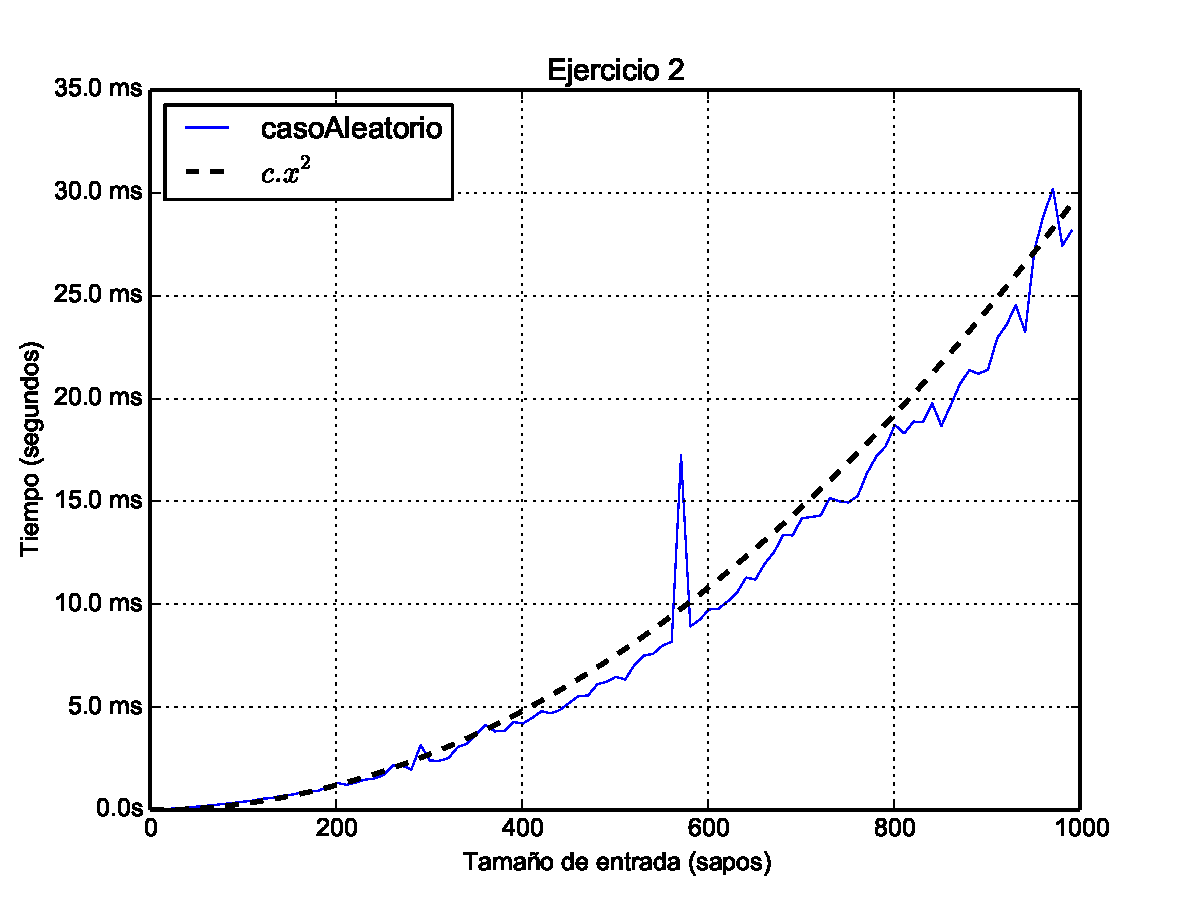
\includegraphics[width=1.4\textwidth, angle=90]{../ej2/graficos/test_tiempoLiso.pdf}
   \caption{\textbf{Muestreo general del Ejercicio 2}}
   \label{fig:ej2-graf-1}
   \end{center}
\end{figure}
\clearpage


\begin{figure}[H]
   \begin{center}
   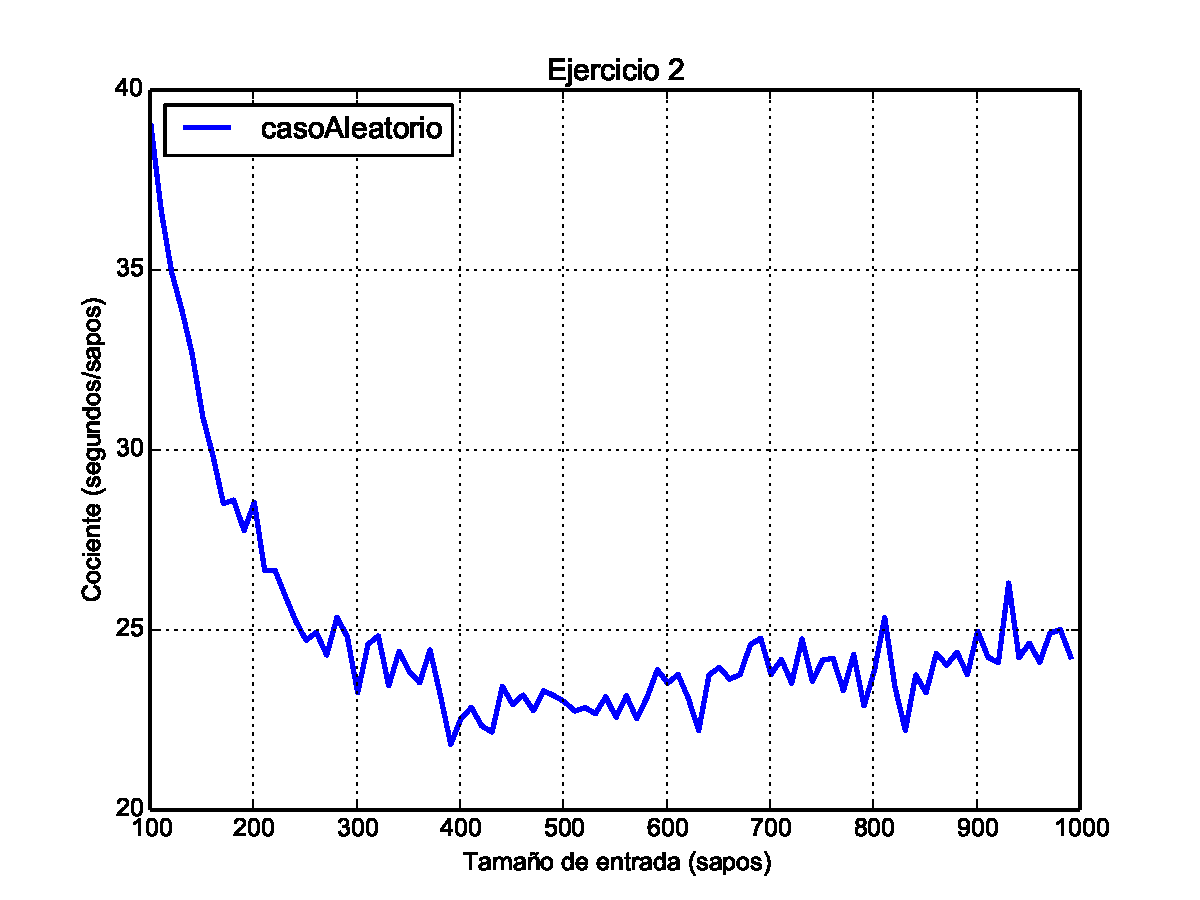
\includegraphics[width=1.4\textwidth,angle=90]{../ej2/graficos/test_Division.pdf}
   \caption{\textbf{Tiempo de ejecución sobre tamaño de la entrada.}}
   \label{fig:ej2-graf-2}
   \end{center}
\end{figure}
\clearpage

Por último, nos pareció interesante realizar una medición de tiempos en función de $k$ (cantidad total de centrales). 
Para este test, las coordenadas de los $n$ pueblos fueron tomadas aleatoriamente, se fijó un $n$ lo 
suficientemente grande, y se midieron los tiempos mientras se variaba el valor de $k$. 
Cuanto mayor sea la cantidad de centrales, la cantidad de conexiones a realizar entre los pueblos es menor, ya que 
como mucho habrá $n - k$ tuberías. Por lo que el tiempo de ejecución del programa disminuiría. 
Si $k = n$ por ejemplo, simplemente se colocaría una central en cada uno de los $n$ pueblos y no haría falta 
ninguna tubería entre ellos.\\
Es evidente, como queda demostrado en la sección de complejidad teórica, que el tiempo de ejecución de nuestro algoritmo es inversamente proporcional a la cantidad de centrales permitidas.
 

% gráfico 3 
\begin{figure}[H]
   \begin{center}
   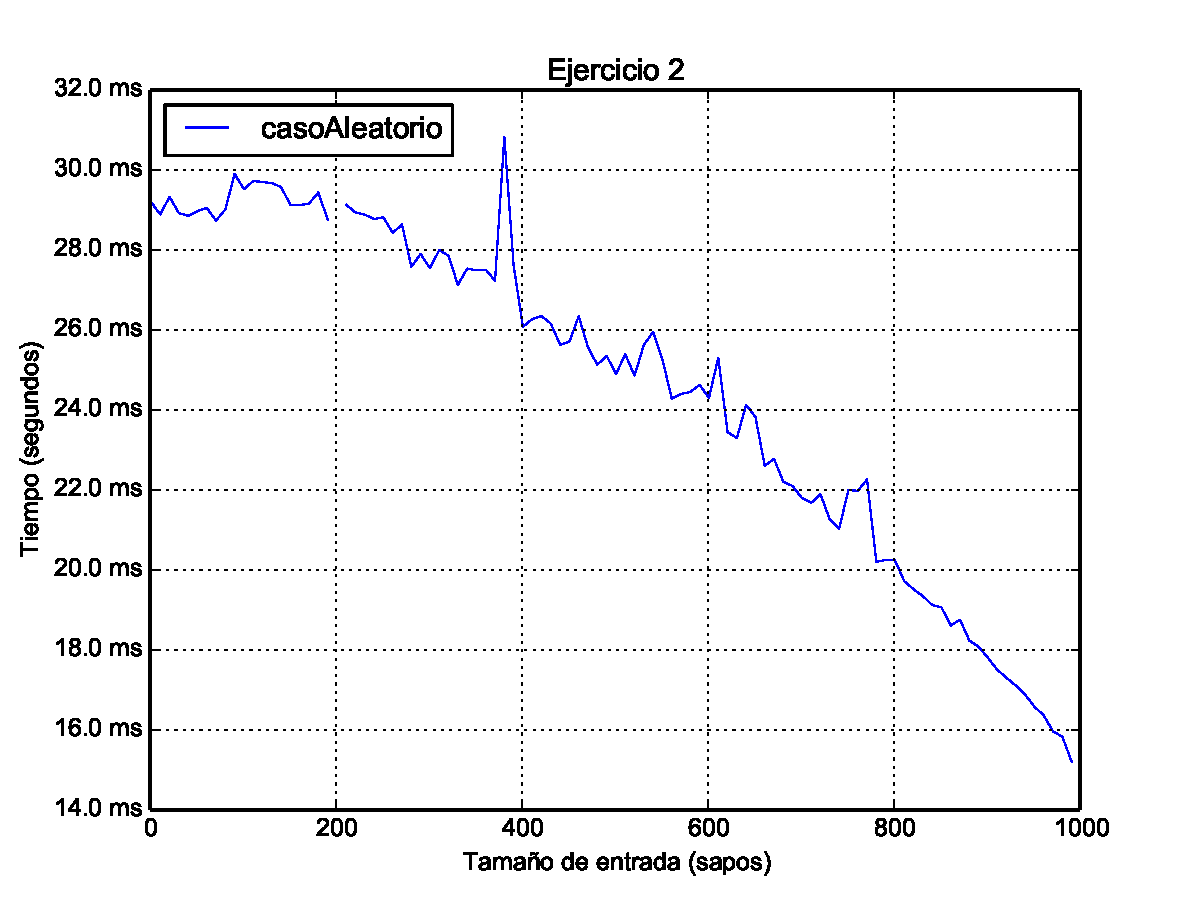
\includegraphics[width=1.4\textwidth,angle=90]{../ej2/graficos/test_variarCantidadCentrales.pdf}
   \caption{\textbf{Tiempo de ejecución en función de la cantidad de centrales ``ITA'' de gas.}}
   \label{fig:ej2-graf-3}
   \end{center}
\end{figure}
\clearpage
   

\end{document}
% -----------------------------------------------
